\picturechapterr{Combining cross-linking mass spectrometry and complexome profiling to structurally characterize mitochondrial protein complexes} \label{ch-1}
%
{
    \begin{center}
        \vspace*{3.5cm}
        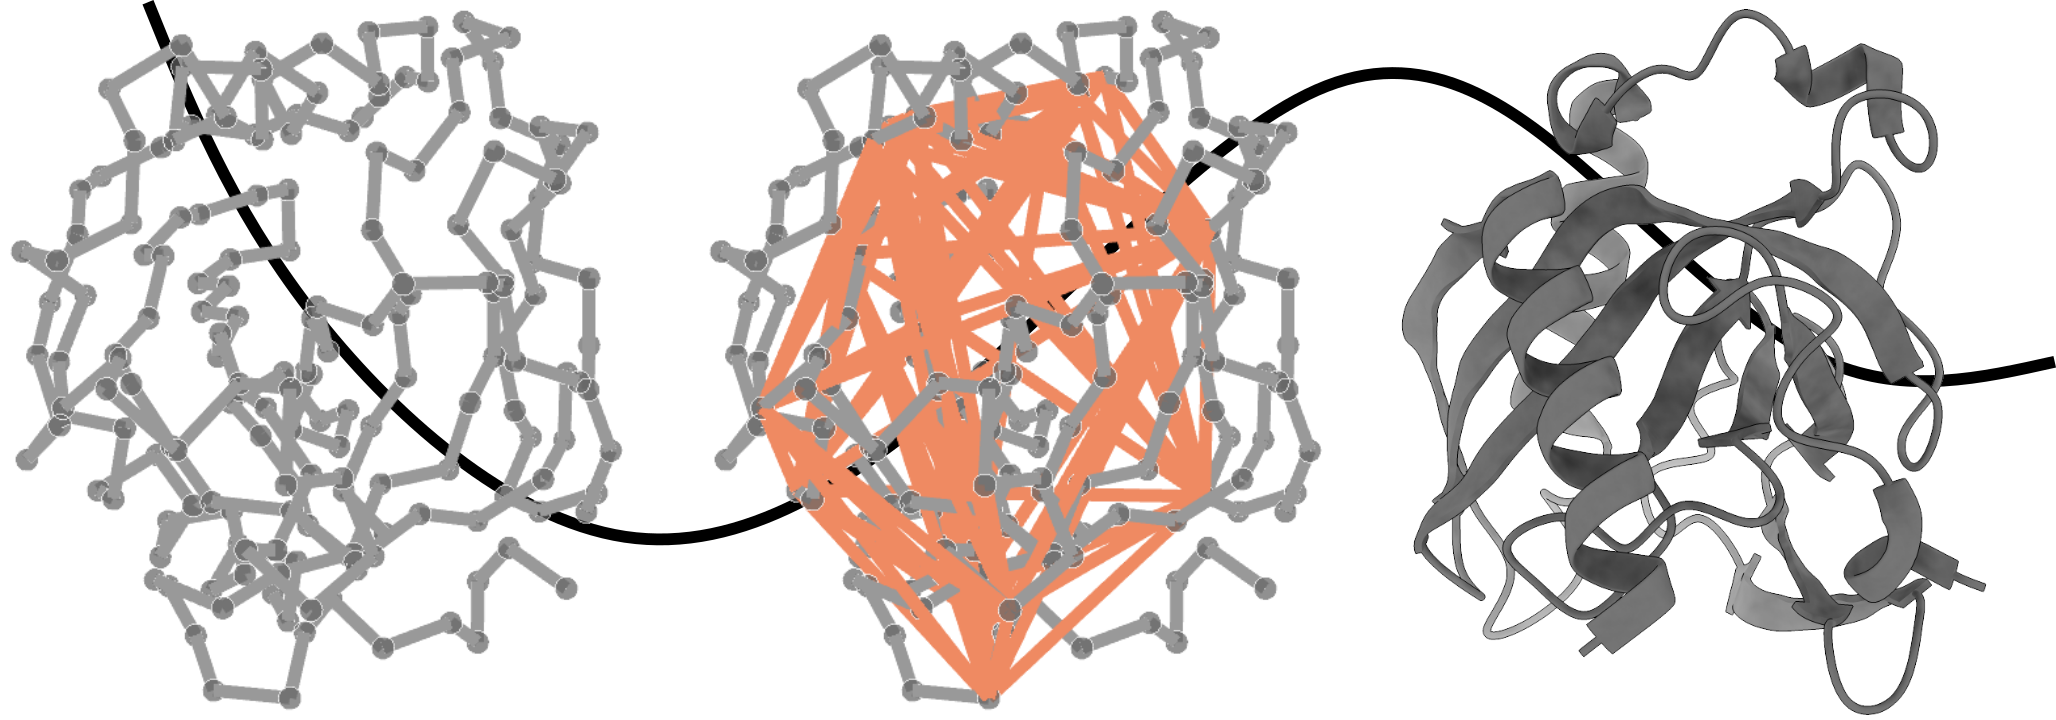
\includegraphics[]{Chapter.1/Figures/chapter1_cover.png}
        \vspace{0.25cm}
    \end{center}
}
%
\begin{flushleft}
    \vspace*{\fill}
    \rule{\textwidth}{1pt}\\[0cm]
    This chapter includes parts of the following publication:\\
    \textbf{Complexome profiling - exploring mitochondrial protein complexes in health and disease}\\
    \footnotesize
    \vspace{0.3cm}
    Alfredo Cabrera-Orefice, Alisa Potter, Felix Evers, Johannes F. Hevler and Sergio Guerrero-Castillo \\
    %\vspace{0.3cm}
    \textbf{\emph{Front Cell Dev Biol.}} (2022), 9:796128, doi: 10.3389/fcell.2021.796128. \emph{Review}\\
\end{flushleft}
\newpage
%
\section{Prelude - The importance of probing protein interactions}
\lettrine[lraise=0.1, nindent=0em, slope=-.5em]{P}{roteins}, the so-called “workhorses” of life, are the tools that make living machines work  \cite{Adams_2008}. The vast majority of biological processes are thus structured, mediated and executed by these macromolecules. Even though many single proteins do perform specific functions by their own, most proteins habitually interact with other proteins, DNA, RNA and lipid molecules rather than acting individually for achieving their biological tasks. The resultant protein complexes can form transient or steady interactions, which also correlate with the type of biological processes they are involved in \cite{De_Las_Rivas_2010}. For example, housekeeping cell processes are likely performed by a large fraction of physically stable protein complexes, whereas in signaling, cell migration, membrane trafficking, metabolic response and other highly dynamic processes, involvement of transient complexes is required for rapid responses and adaptation. The entire set of multi-protein complexes in a cell or compartment is referred to as the complexome \cite{Ceulemans_2006, Deshaies_2002, Lasserre_2006}.

In situations where impaired interaction of the elements of a protein complex affects its proper formation; e.g., due to genetic mutations, the related cell process(es) could be compromised and result in biological dysfunction. Higher complexity in multicellular organisms is of course accompanied by larger complexomes than those from unicellular species. Therefore, alterations in protein complexes may affect not only multiple cell processes, but also lead to severe pathophysiological issues at the tissue/organ level. An integral elucidation of both complexomes and protein interaction networks; i.e., interactome \cite{Vidal_2011} under different cellular scenarios, becomes crucial to fully comprehend the molecular mechanisms behind cell physiology and disease.

Numerous biochemical, biophysical, structural, genetic, microscopy and mass spectrometry (MS) approaches have been applied to characterize protein complexes. Although these methods have different principles, in most cases, they require experimental interventions, cell/tissue fractionation, protein extraction and/or time-consuming protocols prior to data collection and analyses. Besides, the amount of information obtained is often limited to one or a small set of protein complexes. The recent breakthrough in quantitative high-throughput technologies and bioinformatic tools has substantially increased the efficiency and quality of the large-scale identification of protein interactors \cite{Iacobucci_2021, Low_2021}. Accordingly, an outstanding volume of evidence on the composition, 3D structure, interactions and molecular roles of hundreds of protein complexes is now easily accessible through multiple repositories, such as RCSB PDB \cite{Burley_2021}, STRING \cite{Szklarczyk_2021}, CORUM \cite{Giurgiu_2019}, BioGRID \cite{Oughtred_2021}, Pfam \cite{Mistry_2021}, Complex Portal \cite{Meldal_2021}, NCBI \cite{Coordinators_2016} and UniProt \cite{UniProt_2021}. Yet, a substantial fraction of the protein interactors reported in those databases still lack full validation of their occurrence \emph{in vivo} by using novel and more reliable methods.

Further, function and capability to interact is closely linked to a proteins three-dim\-ensional conformation. As such, interrogating structures and interactions of proteins is key to understand cellular processes and therefore has evolved into a significant area of biological research \cite{De_Las_Rivas_2010, Russell_2004}. Discerning structural details of proteins and macromolecular complexes is performed using techniques such as X-ray crystallography, nuclear magnetic resonance (NMR), Small Angle X-ray Scattering (SAXS), cryo-transmission electron microscopy (cryo-EM) as well as cryo-electron tomography (cryo-ET) \cite{Cerofolini_2019, Dunstone_2017}. Especially, X-ray crystallography, NMR and cryo-EM with the ability of providing atomic structures of proteins and protein complexes contributed unprecedented structural and biological insights into processes crucial for cellular life \cite{Cate_1999, Englmeier_2019, O'Connell_2009}. Despite these accomplishments, these more standard techniques also have their limitations. Foremost, they predominantly require a highly purified sample for analysis, consequently proteins and protein complexes are rarely studied in their naïve cellular environment. In recent years it has become very apparent that structures need to be solved \emph{in situ} to fully understand biological processes, but methods enabling \emph{in situ} structural characterization lagged behind \cite{Lucic_2008}. Opposing the reductionist approach, cryo-ET allows to image whole organisms, tissues, cells and organelles. Recorded images are subsequently reconstructed into three-dimensional tomograms, enabling the investigation of macromolecular complexes in a near native environment \cite{Doerr_2017}. Although cryo-ET holds a future potential to image the entire proteome of a cell, it is currently still limited to highly abundant, very large protein complexes such as ribosomes or respiratory chain assemblies \cite{Davies_2014, Turk_2020}. Alternatively, mass spectrometry (MS) allows to study macromolecules and their assemblies independent of their size and abundance and has thereby evolved into a new pillar in the structural characterization of the proteome (structural proteomics). Since the development of electrospray ionization (ESI) \cite{Fenn_1989, Yamashita_1984} and matrix-assisted laser desorption ionization (MALDI) \cite{Karas_1988} in the mid 1980's, rapid technical advancements resulted in a diverse suit of MS-based techniques for the structural characterization of proteins and protein assemblies. A selection of popular structural MS methods is depicted in \textbf{\autoref{fig:fig1}}. The diversity of available methods not only arose from the many different macromolecules present in the proteome but also from different analysis strategies. Fundamentally, MS-based approaches can be divided into protein-centric and peptide-centric strategies \cite{Soldi_2013}. While protein-centric strategies enable the characterization of intact proteins and protein complexes, peptide-centric approaches delineate structural information by enzymatically digesting proteins into peptides prior to MS analysis. Despite those differences, MS based methods can provide highly complementary structural information on proteins and protein complexes such as their conformation, post-translational modifications (PTMs), surface properties, interaction interfaces, stoichiometry and subunit connectivity. Especially in combination with computational modeling, MS based technologies provide a toolbox that is helpful to unravel structural details that would not be easily accessible with other structural approaches.

\begin{figure*}[hbt]
    \center
    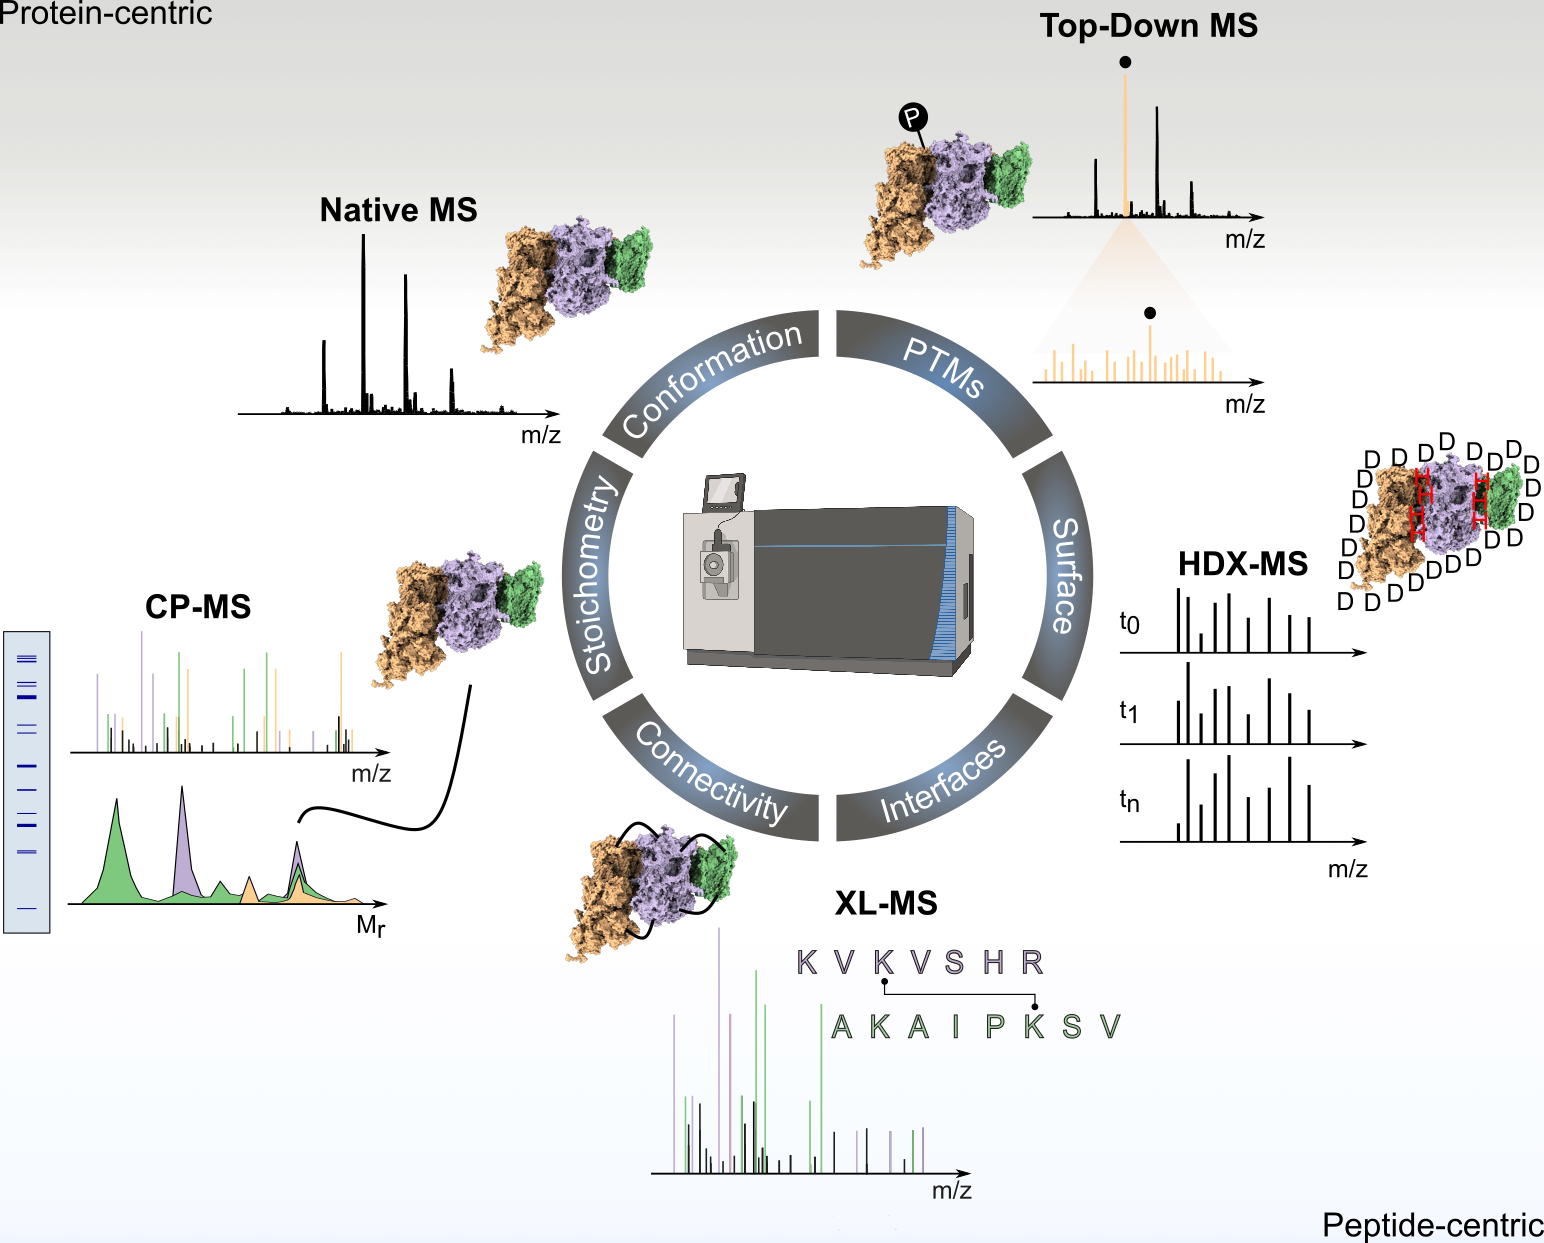
\includegraphics[]{Chapter.1/Figures/Figure1.png}
    \caption{\textbf{Overview of various types of structural MS techniques that can be applied for the characterization of proteins and protein complexes.} The top panel describes protein-centric approaches (native-MS, top-down MS), where intact proteins are analyzed. Complementary, peptide-centric methods (XL-MS, CP-MS, HDX-MS) depicted in the bottom panel, delineate structural information of proteins and protein complexes from peptides.}
    \label{fig:fig1}
\end{figure*} \clearpage
Amongst the versatile MS based toolbox, cross-linking mass-spectrometry (XL-MS) and complexome profiling mass-spectrometry (CP-MS) have emerged as powerful methods to structurally and functionally characterize proteins and protein-protein interactions \cite{Steigenberger_2020}. Nonetheless, both methods also present drawbacks that significantly hamper an adequate structural characterization of protein assemblies. In this thesis I present a collection of XL-MS based advancements that significantly improve the structural and functional analysis of protein complexes in mitochondria. In short, chapter 2 and 3 introduce XL-MS and CP-MS as highly complementary methods, allowing the detailed characterization of protein complexes. Chapter 4 and 5 highlight how XL-MS can aid the identification and characterization of protein complexes using cryo-ET as well as computational structure prediction methods. In the subsequent parts of this introduction, I will succinctly review the fundamentals of XL-MS and CP-MS. The last part will be devoted to how XL-MS in combination with CP-MS and computational modeling, whereby I describe how such a combination can benefit our molecular understanding of mitochondrial protein complexes.
%
\section{The fundamentals of probing protein structure and interactions with XL-MS}
Chemical cross-linking is a special category of protein chemical modifications, and as such it was developed already over 70 years ago to elucidate the chemical and biological function of proteins \cite{French_1945}. Using a cross-linking reagent non-covalent interactions within or between amino acid side-chains of proteins are converted into covalent chemical bonds, stabilizing proteins or protein complexes so that they can be analyzed using methods that normally could denature proteins \cite{Means_1998, Naowarojna_2021}. Like that, cross-linking paired with gel electrophoresis enabled the identification of protein-protein interactions in ribosomes of \emph{Escherichia coli} as early as in the 1970s \cite{Clegg_1974, Sun_1974}. The development of peptide-centric MS methods roughly 30 years later substantially increased the impact of cross-linking for the structural characterization of proteins and respective complexes \cite{Rappsilber_2011, Rappsilber_2000}. Combining cross-linking and peptide-centric MS (XL-MS) enabled not only the fast and sensitive identification of cross-linked proteins but furthermore promised to reveal the position of interacting residues, thereby catering valuable restraints for the structural characterization of proteins and protein complexes. Advances in instrumentation, bioinformatics tools as well as the development of innovative-, MS compatible cross-linkers further increased the application of XL-MS, for instance to study also protein-nucleic acid interactions \cite{Gotze_2021, Wong_1991}.
%
\subsection*{An overview of available cross-linking reagents}
To date, a variety of MS compatible cross-link reagents have been introduced, all aiming at efficiently leveraging spatial distance restraints representative of the in-solution state of proteins and protein complexes. To accomplish this, most of the available reagents typically share a similar structural design, in which two reactive moieties (most commonly amine-reactive) are connected by a spacer arm. However, to account for different applications, e.g. different type of samples as well as to ease the identification cross-linked peptides more elaborated designs have been developed \cite{Steigenberger_2020}. To counteract the low efficiency of the cross-linking reaction, and the subsequent low abundance of cross-linked peptides \cite{Leitner_2014, Leitner_2010}, cross-linkers containing enrichable moieties have been introduced. The usage of linkers with enrichable handles like biotin, phosphonic acid as well as azides proved to significantly increase the number of detected cross-linked peptides, by reducing the huge background of non-modified peptides \cite{Matzinger_2020, Steigenberger_2019, Tan_2016}. Additionally, to simplify the computational challenges that are accompanied with identifying cross-linked peptides, so-called “cleavable” cross-linkers have been introduced. Cleavable-cross-linkers possess a labile moiety between the two reactive groups, which can be cleaved during MS analysis. This reduces the subsequent MS2 sequencing to just a single precursor mass originating from an individual peptide with respective part of the cross-linker attached. In contrast, “non-cleavable” cross-linkers stay intact during MS analysis for which subsequent spectra contain fragment ions of the two linked peptides which significantly hampers the identification \cite{Kao_2011}. A more detailed explanation of MS identification of cleavable and non-cleavable cross-linked peptides will follow below.

\begin{figure*}[hbt]
    \center
    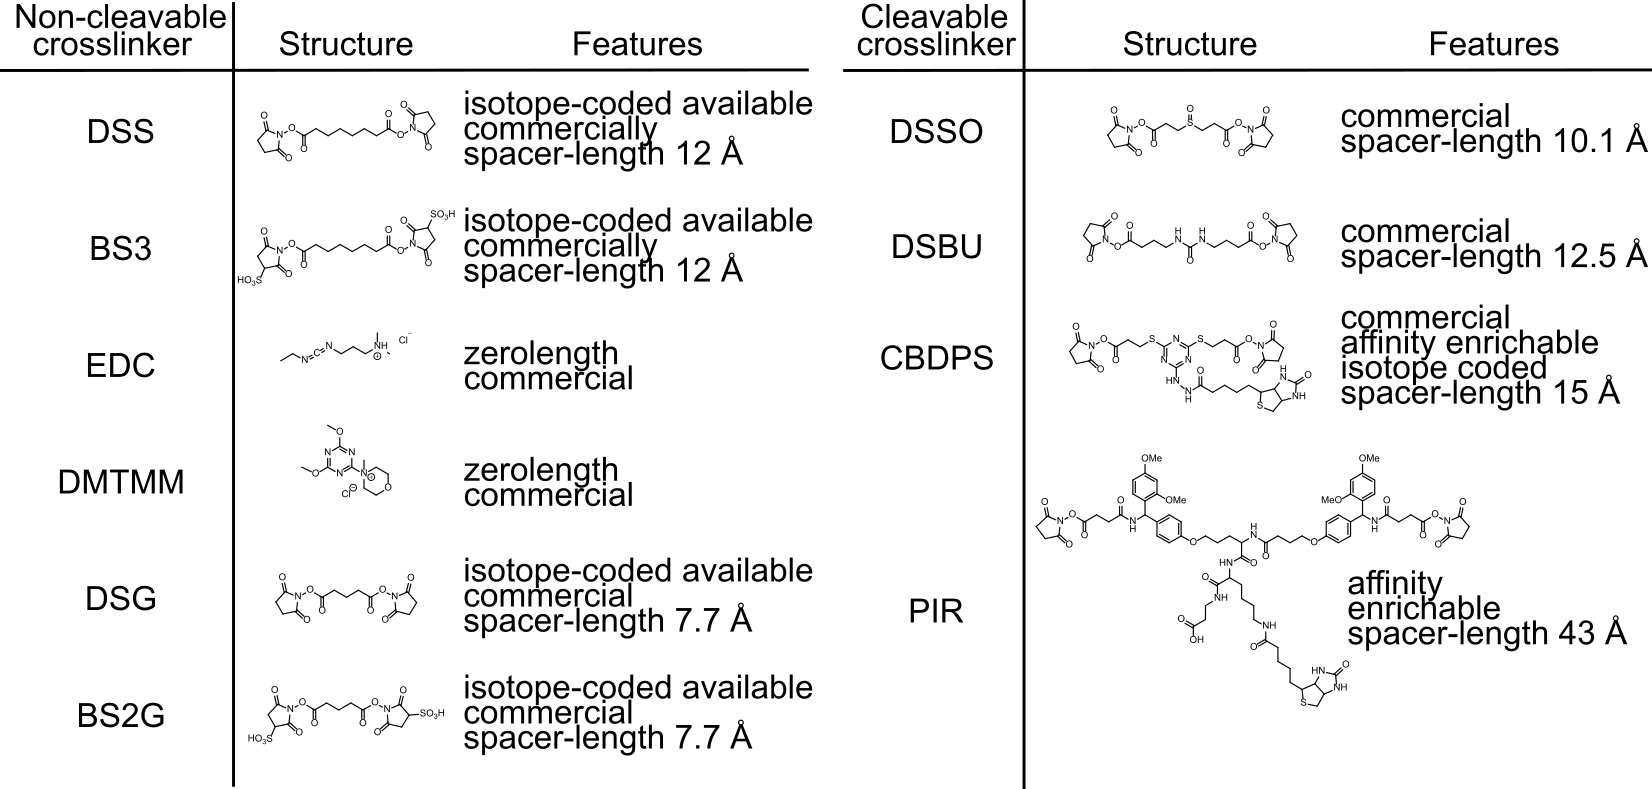
\includegraphics[]{Chapter.1/Figures/Figure2.png}
    \caption{\textbf{Overview of MS-compatible cross-linking reagents.} Figure adapted with permission from \cite{Steigenberger_2020}}
    \label{fig:fig2}
\end{figure*}
Lastly, to further increase the stringency for produced distance restraints, so called “zero-length” cross-linkers have been introduced. These compounds mediate the direct conjunction of two proximal residues with no intervening spacer arm or linker. This theoretically reduces the produced distance restraints to only the length of the side chains ($\sim$15 Å), as opposed to cross-linkers with a spacer arm that produce distance restraints >25 Å. Limiting possible residue-residue distances is especially beneficial when utilized as constraints in computational modelling of proteins or protein complexes, as it reduces the number of possible orientations \cite{Leitner_2014}. An overview of some of the more commonly used cross-linkers is depicted in \textbf{\autoref{fig:fig2}}.
%
\subsection*{XL-MS to characterize protein-protein interactions in mitochondria}
Most cross-linking studies are performed on purified proteins and protein complexes, however in recent years an increasing amount of applications have been reported for more complex systems like whole organelles, cells and even tissue as reviewed in for instance \cite{O'Reilly_2018}. An advantage of working with purified proteins and protein complexes is the significantly simplified detection and identification of cross-links using MS including a more straightforward data analysis. Notwithstanding the challenge, only XL-MS studies of naive systems such as intact mitochondria, can provide a comprehensive interaction network thereby enabling a better understanding of biological processes and dependencies. To tackle the complexity of such systems, several technical and experimental advancements have been presented over the past years enabling the successful identification of mitochondrial protein interactions using XL-MS \cite{Liu_2018, Ryl_2020, Schweppe_2017}.  Given the complexity of mitochondrial proteomes, the selection of a suitable cross-linker, prior to MS-analysis is essential (\textbf{\autoref{fig:fig3}A}). Gas-phase cleavable cross-linkers such as DSSO \cite{Kao_2011} or cross-linkers with an enrichment handle such as PhoX \cite{Steigenberger_2019} significantly simplify the subsequent identification of the XLs. Although NHS- reactive cross-linkers, covalently linking proximal lysine-side chains, are still most commonly applied in cross-linking experiments \cite{Steigenberger_2020}, cross-linkers with an alternative side-chain reactivity are valuable reagents to increase the cross-link coverage. The zero-length cross-linker DMTMM, which promotes the condensation between carboxyl-groups (Glutamic acid, Aspartic acid) and primary amines (Lysines) can increase the cross-linking coverage of membrane proteins, as hydrophobic patches which typically carry none or very few Lysine residues could be targeted via Glutamic acid and Aspartic acid residues \cite{Hevler_2021b}. Importantly, before each application, cross-linking conditions, e.g. the ratio of cross-linker to protein or choosing of a suitable cross-linking buffer, need to be carefully optimized \cite{O'Reilly_2018}. After cross-linking, mitochondria are disrupted either mechanically (e.g. sonication) or by using detergents (e.g. Triton-X-100) and soluble proteins are subsequently denatured, reduced, and alkylated, alike in standard bottom-up proteomics experiments. Before enzymatic digestion of soluble proteins into peptides, contaminations such as lipids and detergents are removed by precipitation or phase extraction \cite{Klykov_2018}. After digestion, cross-linked peptides, which can either stem from the same protein (intra cross-link) or from two distinct proteins (inter cross-link), are significantly less abundant than their “linear” (non cross-linked) and “mono-linked” counterparts \cite{Leitner_2014, Leitner_2010, Sinnott_2020} (\textbf{\autoref{fig:fig3}B}). Mono-linked peptides are linear peptides which carry the cross-linker that is quenched or hydrolyzed on the other reactive group rather than attached to another peptide. In contrast to linear peptides, mono-linked peptides contain structural information and are commonly used to assess protein surface accessibility as well as to support scoring of structural models \cite{Sinnott_2020}. The sub-stoichiometric reaction efficiencies render the identification of cross-linked peptides challenging, especially in complex samples such as intact cell and mitochondria. To obtain satisfactory identification of cross-linked peptides relative to their linear counter parts, an enrichment step is often essential (\textbf{\autoref{fig:fig3}C}). Enrichment most often takes place via chromatographic methods, such as strong-cation-exchange (SCX) fractionation, that can be used to separate doubly charged linear (tryptic) peptides (carrying a charge at the N and C terminus) from higher charged, cross-linked peptides (typically carrying double the number of charges). In case an enrichment handle such as a phosphonate group (PhoX) is used, cross-linked peptides can be captured onto a suitable material (e.g. Fe3+ IMAC), thereby allowing the separation from linear peptides. After enrichment, cross-linked peptides are identified following different MS acquisition strategies (\textbf{\autoref{fig:fig3}D}). Which MS acquisition method to use, is largely determined by the applied cross-linker \cite{Liu_2017a}. Lastly, recorded XL-MS spectra can be searched using various software suits
\begin{figure*}[p]
    \center
    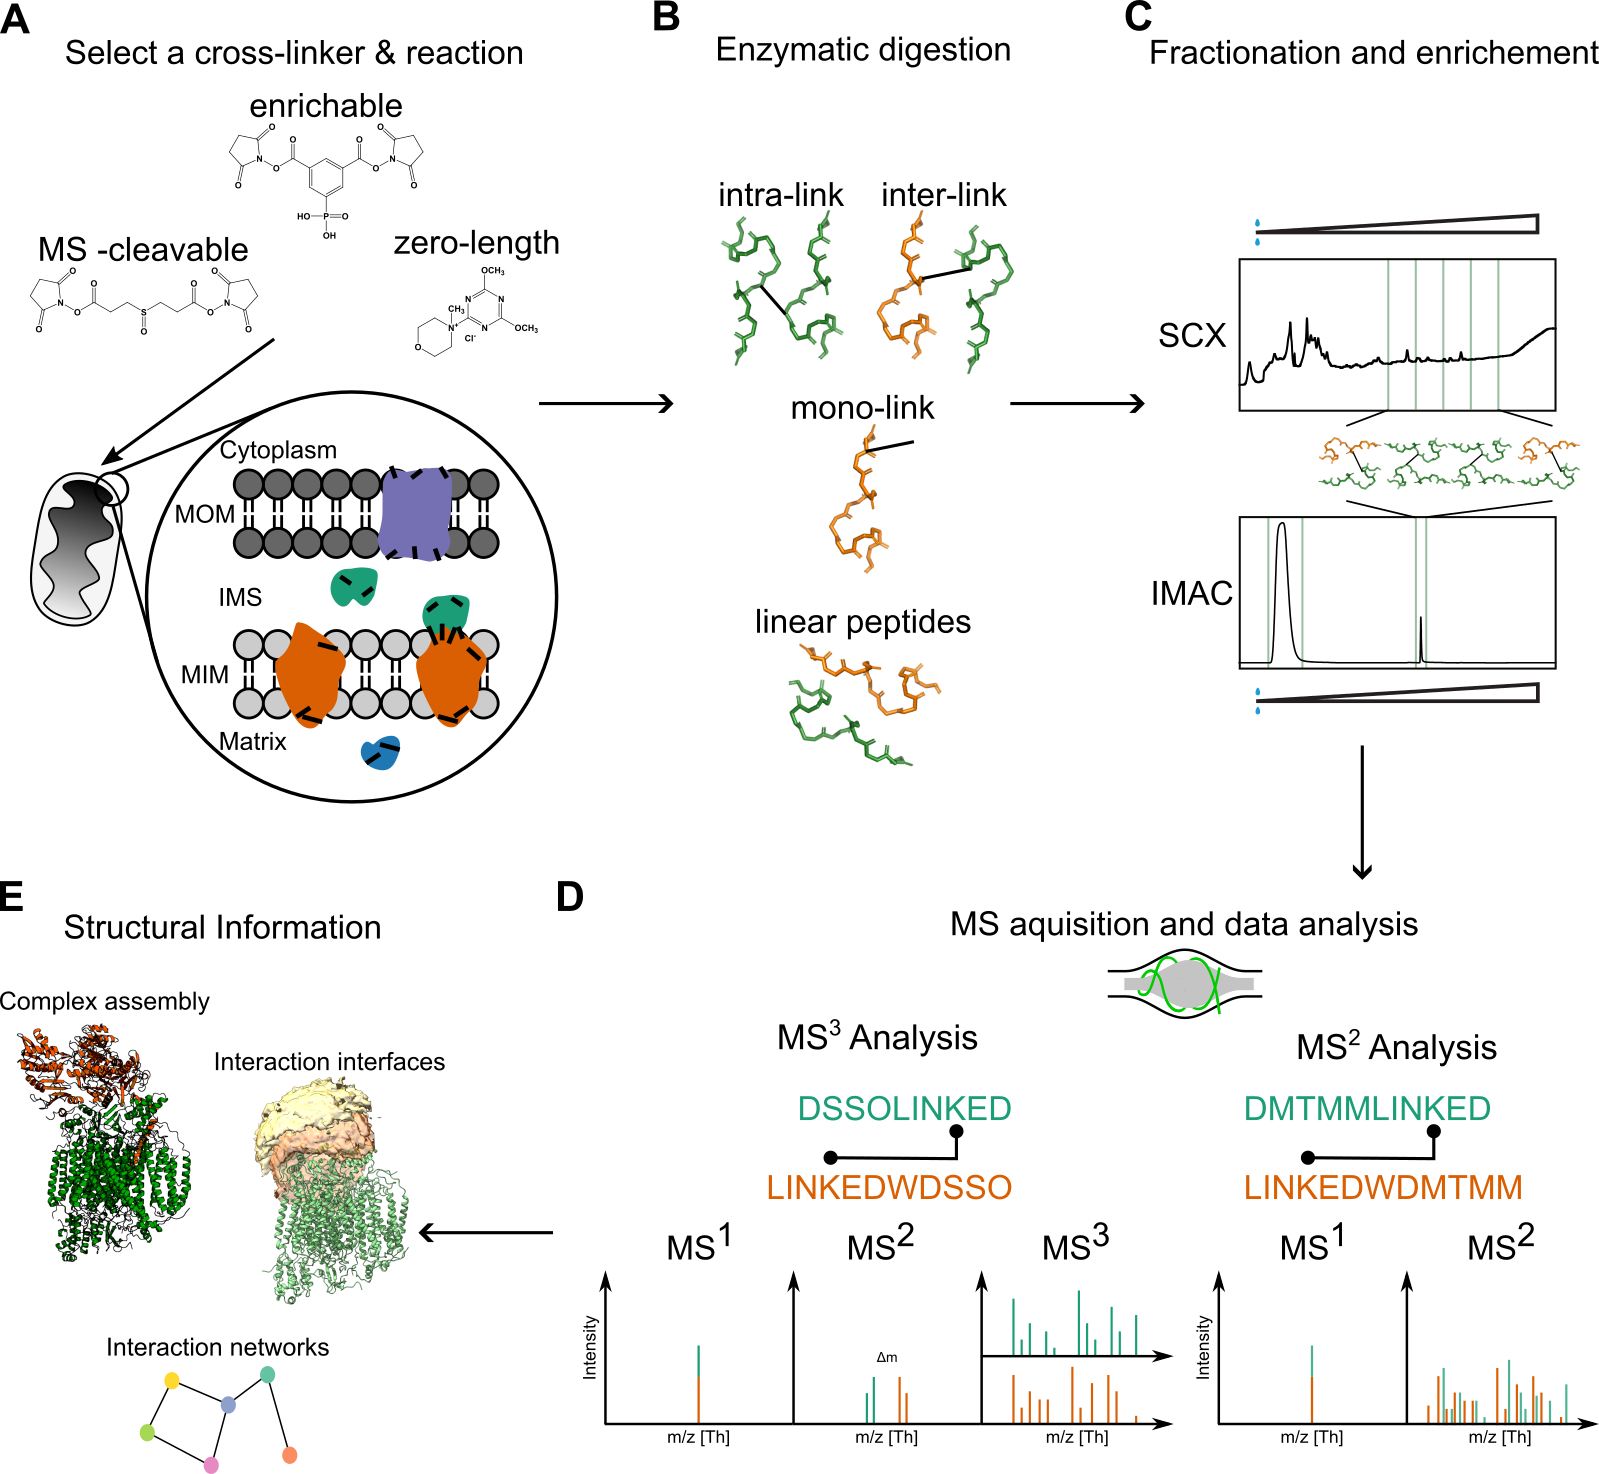
\includegraphics[width=0.95 \textwidth]{Chapter.1/Figures/Figure3.png}
    \caption{\textbf{Experimental strategies for the analysis of proteome-wide protein-protein interactions in mitochondria.} \textbf{A.} Cross-link reagents comprise various chemistries as highlighted in \textbf{\autoref{fig:fig2}}. For cross-linking mitochondria, reagents with a cleavable spacer arm, enrichable handle or an alternative amino-acid reactivity are beneficial to increase the number of cross-link identifications. DSSO is depicted here as an example for a cleavable cross-linker. PhoX is depicted as an example for a cross-linker with an enrichment handle (phosphonic acid) and DMTMM is depicted as example for a zero-length cross-linker. For each application, conditions such as concentration and reaction time need to be carefully optimized to achieve optimal cross-linking. \textbf{B.} After solubilization of mitochondrial membranes proteins are enzymatically digested, producing a mixture of cross-linked and linear peptides. Cross-links can be formed within protein sidechains (intra link) and between sidechains of different proteins (inter link). Additionally, linear peptides with the cross-linker attached (mono-links) can be formed. \textbf{C.} To increase MS identification, cross-linked peptides are separated from linear peptides using chromatographic methods, such as strong-cation-exchange chromatography (SCX) or Fe3+ IMAC enrichment chromatography. \textbf{D.} Depending on the chosen cross-linker (e.g. gas-phase cleavable or non-cleavable) different MS acquisition strategies can be applied, to increase the likelihood of identifying a cross-linked peptide. \textbf{E.} Different software solutions as described in the text can be utilized to identify linked peptides. Information of cross-linked experiments can be used to elucidate protein-protein networks, interaction interfaces as well as to structurally model protein complex assemblies as described in the text. Figure adapted from \cite{Hevler_2021b}.}
    \label{fig:fig3}
\end{figure*}
such as pLink2 \cite{Chen_2019b}, MeroX \cite{Gotze_2015}, StavroX \cite{Gotze_2012}, Xi \cite{Chen_2019a}, Kojak \cite{Hoopmann_2015} and XlinkX \cite{Klykov_2018}. However, not all software solutions are capable of analyzing all MS-acquisition strategies or cross-link reagents (e.g. MS3, DSSO), as such software capability as well as availability should be taken into consideration when designing a XL-MS experiment. Likewise, methods for FDR calculations might differ across platforms, thereby impacting the quality and ambiguity of outputted XL-MS results \cite{Matzinger_2022}. Careful manual validation of identified cross-linked peptides is still advisable before utilizing them for the structural characterization of protein complexes (\textbf{\autoref{fig:fig3}E}). Strategies for MS-acquisition, and applications of XL-MS for structural characterization of proteins and protein complexes will be further discussed in the following sections.
%
\subsection*{XL-MS-data acquisition}
In classical bottom-up proteomics, linear peptides are identified based on their accurate mass (measured at the MS1 level) and sequence specific fragment ions (measured at the MS2 level). To be analyzed within the mass spectrometer, peptides are first ionized and thereby separated from their carrier medium (usually aqueous or organic phase). Charged and ionized peptides are next transmitted into the mass spectrometer, where the mass of the intact peptide-ion is determined by a mass analyzer (MS1 signal). The mass of each ion is measured by monitoring their motion through the mass analyzer, which is dependent on the mass to charge ratio (m/z). Work presented in this thesis utilized instruments equipped with quadrupoles, linear ion traps (LIT) as well as an Orbitraps as mass analyzers. To confidently determine the correct peptide sequence, the peptide ion is fragmented inside the mass spectrometer providing additionally m/z values for its fragment ions (MS2 level). Depending on the fragmentation technique used, different fragment ions corresponding to cleavage of the peptide backbone can be observed. Most frequently, collision-induced dissociation (CID) \cite{Hunt_1986} and higher-energy C-trap dissociation (HCD) \cite{Olsen_2007} fragmentation techniques are applied, producing b and y fragment ions that reflect N- and C-terminal fragments, respectively being cleaved at the peptide bonds. For XL-MS applications, further fragmentation of an isolated fragment ion (MS3 level) can be very useful, however not all mass spectrometers are capable of performing such higher order, e.g. MS3, experiments \cite{Liu_2017a, Lossl_2016}.\\
For XL-MS experiments, the seemingly well-established MS analysis for the identification of linear tryptic peptides is substantially impaired, due to the fact that the cross-linked peptide is composed of two covalently bound linear peptides. As such, the two peptide moieties presents in these cross-linked peptide precursor ions are normally co-fragmented in the same MS2 spectra, often with different fragmentation efficiencies for the two peptide moieties hampering the full identification of both \cite{Liu_2017a}. To circumvent impaired fragmentation and to increase the fragmentation efficiency, cross-linked peptides are commonly fragmented using multiple collision energies (CID/HCD), resulting in more informative fragmentation spectra (MS2 method). Importantly, also the cross-link reagent moiety can impact the fragmentation. Consequently, collision energies need to be optimized for each cross-linker to obtain the best fragmentation efficiency. Likewise, combining complementary dissociation methods such as CID/HCD and electron transfer dissociation (ETD) can be applied for an improved fragmentation (MS2-MS2 method) \cite{Campbell_2009, Frese_2012, Liu_2017b} (see \textbf{\autoref{fig:fig3}D}). Additionally, gas-phase cleavable cross-linkers \cite{Sinz_2017}, such as DSSO have been developed to address such impaired fragmentation. Such cross-linkers are cleaved during the fragmentation process of the XL peptide ions inside the vacuum of the mass analyzer, thereby enabling the dissociation of the cross-linked peptides and greatly improving fragmentation and thus cross-link identification of the two peptide moieties \cite{Liu_2017a}. When measuring on mass spectrometers capable of MS3 analysis, a dual-fragmentation strategy for cleavable cross-linkers can be applied. In such an approach, a survey scan (MS2) is performed, in which a dissociation energy is chosen that specifically breaks the cleavable cross-linker thereby giving rise to signature ions with a unique mass difference corresponding to the cleaved cross-linked peptide each with a part of the cross-link moiety attached. Whenever the mass spectrometer identifies the XL-peptide signature ions, a subsequent isolation and fragmentation step is performed to obtain better sequence information (MS3 analysis) \cite{Liu_2017a, Sinz_2017} (see \textbf{\autoref{fig:fig3}D}). The utilization of gas-phase cleavable cross-linkers in combination with MS3 acquisition strategy has been found to be extremely useful for the analysis of proteome-wide XL-MS experiments such as cell lysates \cite{Klykov_2018, Liu_2017a} as well as intact organelles such as mitochondria \cite{Liu_2018} or nuclei \cite{Fasci_2018}. Notwithstanding, it was recently shown that MS2- and MS2-MS2 acquisition methods can outperform MS3 acquisition strategies in terms of unique crosslink numbers \cite{Matzinger_2022}, suggesting that the new generation of MS2 capable mass-spectrometers can also be used for analysis of proteome-wide, gas-phase cleavable XL-MS experiments.
%
\subsection*{Applications of XL-MS for the structural characterization of protein complexes}
Beyond what is well possible using more common techniques in structural biology, XL-MS can also be performed under naïve cellular conditions, reducing possible artifacts that may occur during recombinant expression and/or purification of proteins and protein complexes \cite{Niedzialkowska_2016}. In the latter case additional artefacts may occur during in vitro reconstitution of a protein complex. Additionally, benefits of probing protein-protein interactions \emph{in vivo} have been shown in work on mouse heart mitochondria, for which a number of protein-protein interactions could only be observed in intact mitochondria and not upon membrane disruption \cite{Liu_2018}. XL-MS studies applied to cell lysates or intact organelles such as mitochondria, have successfully captured proteome-wide PPIs, thereby enhancing our understanding of how the proteome is wired \cite{Fasci_2018, Klykov_2018, Liu_2017b, Ryl_2020, Schweppe_2017} (\textbf{\autoref{fig:fig4}A}). While such interaction networks are also commonly generated through other MS based methods such as affinity-purification MS (AP-MS) \cite{Huttlin_2017, Krogan_2006}, intra and inter cross-links generated by XL-MS additionally provide information that can be used for the structural characterization of proteins and protein complexes \cite{Bullock_2018, Klykov_2018, Orban-Nemeth_2018}. Intra protein cross-links provide information about proximal amino acids within a protein, which can be applied as distance restraints in subsequent computational modeling \cite{Orban-Nemeth_2018} (\textbf{\autoref{fig:fig4}B}). Distances for cross-link restraints applied in computational modeling are mostly calculated between C\(\alpha\)-C\(\alpha\), by summing the length of each side chain and the length of the cross-linker. As side-chains and cross-linkers are highly flexible, distance restraints are typically provided as a range (with a minimum and maximum value) rather than a defined distance value. Modeling software`s such as I-Tasser \cite{Yang_2015}, Robetta \cite{Kim_2004} and Modeller \cite{Webb_2016} employ set cross-link constraints for model building as well as for scoring features (e.g. geometry) of the structure which may not be evaluated by standardly used score terms. Recent breakthroughs in the field of protein structure prediction by AI driven tools such as AlphaFold2 \cite{Jumper_2021} and RoseTTA-fold \cite{Baek_2021}, enable the generation of structural models based solely on the amino acids sequence of a protein. However, validation and finding the biological relevant confirmation can be time consuming and challenging with only having the provided output scores at hand. For this, it was recently shown that intra cross-links can be utilized to aid the validation process as well as to pinpoint towards biologically active structural conformations \cite{McCafferty_2022}.

Moreover, \emph{ab initio} protein-protein docking offers a possibility to computationally predict protein complexes and protein-protein interfaces, given that the structures of the individual sub-units are known \cite{Dominguez_2003, Vakser_2014}. For most of the available programs complex
conformations are predicted by rotating and translating one complex component (often the smaller protein) around the other one, which is fixed in space.

\begin{figure*}[htb]
    \center
    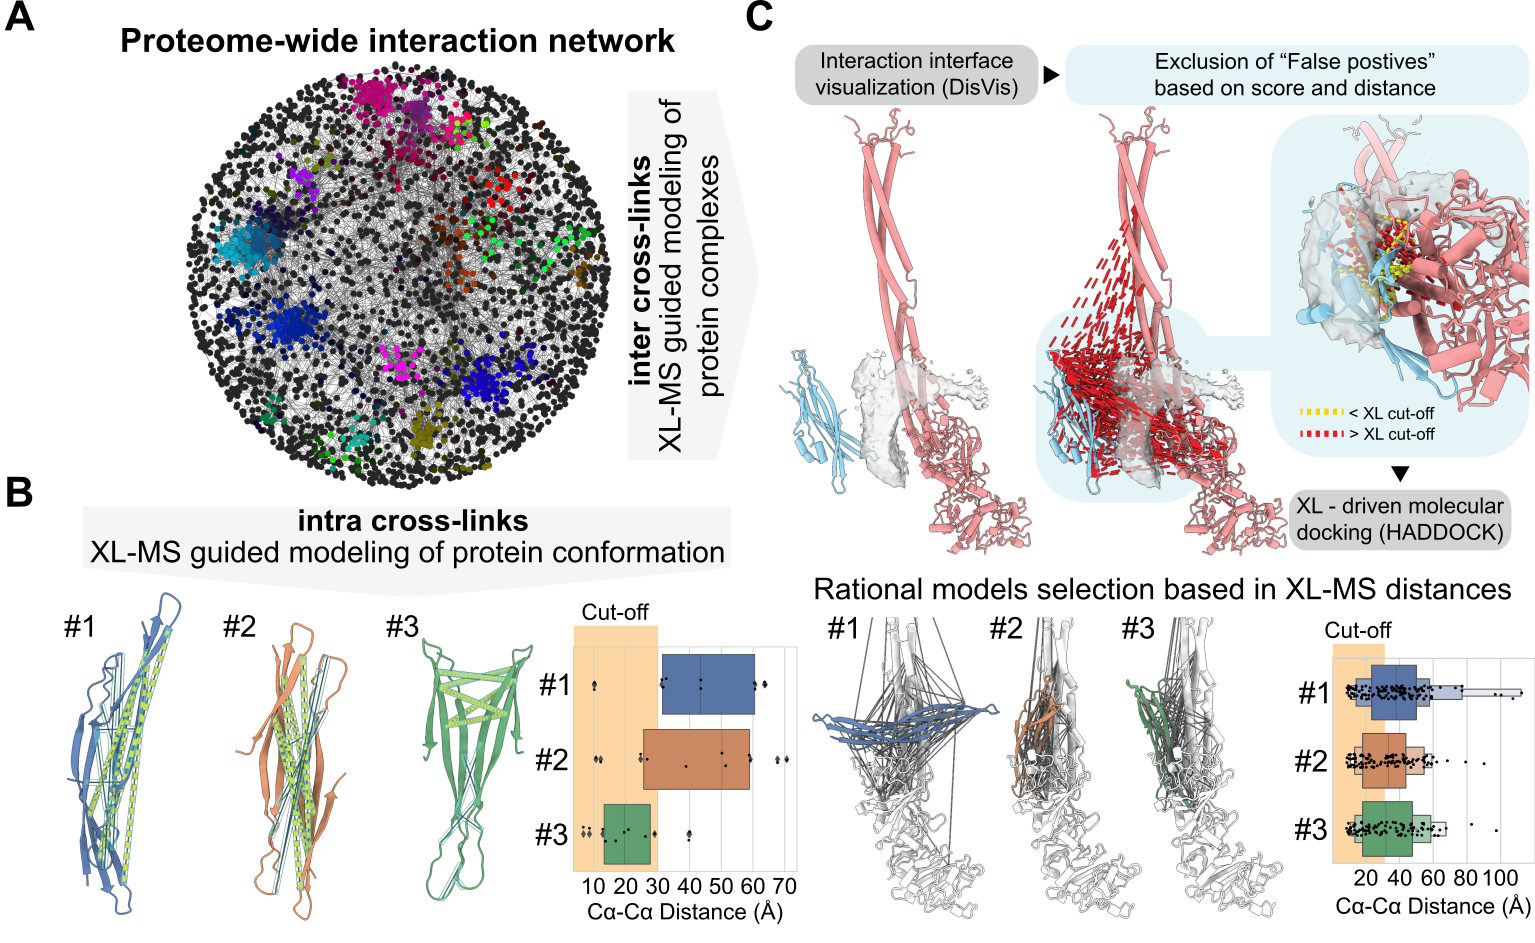
\includegraphics[]{Chapter.1/Figures/Figure4.png}
    \caption{\textbf{Applications of XL-MS for the structural characterization of proteins and protein complexes} \textbf{A.} When XL-MS is applied on high complex samples, such as cell lysates or intact organelles, protein-protein interaction networks can be generated. Protein interaction networks highlight how a soluble proteome is wired. Proteins are shown as black nodes, with proteins that have a similar GO functional annotations \cite{Ashburner_2000} being depicted in bright colors. \textbf{B.} Intra protein cross-links can be utilized to guide structural modeling of a protein conformations, as well as to validate AI derived structural models. \textbf{C.} Inter protein cross-links can be utilized to model protein complexes observed in the interaction network. Information about proximal amino acids is validated and utilized to identify interaction interfaces and active interface residues (e.g. using DisVis \cite{van_Zundert_2015}). True positive inter-crosslinks as well as information about active interface residues can subsequently be used as input for protein-protein docking (e.g. using Haddock \cite{van_Zundert_2016}). Validation of generated complex models can be performed by mapping obtained inter cross-links onto final structures. Figure adapted from \cite{Lagerwaard_2022} with permission. Data to generate the protein-protein interaction network was obtained from \cite{Costanzo_2016}}
    \label{fig:fig4}
\end{figure*}\clearpage
This approach, however, is still very time consuming and computationally expensive as all theoretically possible conformational spaces have to be sampled and scored \cite{Dominguez_2003, van_Zundert_2016}. Inter protein cross-links identified in XL-MS experiments, provide information about the arrangement of proteins within a complex. Utilizing inter cross-links as additional restraints to guide the docking process alongside traditional energetics and shape complementarity can therefore significantly reduce the possible conformational space and increase the chance for the prediction to result in a unique solution \cite{Dominguez_2003, van_Zundert_2016} (\textbf{\autoref{fig:fig4}C}). HADDOCK \cite{Dominguez_2003, Orban-Nemeth_2018} (High Ambiguity Driven protein-protein Docking) is a powerful tool that can make use of biochemical and/or biophysical interaction data such as inter cross-links observed in XL-MS experiments. To utilize cross-links for guiding structural docking, the provided information content needs to be first evaluated. DisVis \cite{van_Zundert_2015} is a software suit enabling the identification of false-positive cross-links as well as the characterization of surface residues that are most often contacted in all possible models (interface residues). True-positive cross-links together with active interface residues are employed as additional restraints to predict a protein complex and later for validation and model selection. Besides guiding protein-protein docking, cross-linking data was shown to benefit other structural and modeling techniques, for instance with the assignment of ambiguous densities in cryo-EM maps \cite{Herzog_2012, Kyrilis_2021b} or with identifying and refining high confidence models predicted for protein complexes based on AI \cite{Burke_2021}.

Although the prime technology used for the work described in this thesis is cross-linking mass spectrometry, several of the chapters involved the use of another powerful approach, namely complexome profiling. Below I describe succinctly also this approach, largely adapted from \cite{Cabrera-Orefice_2022}, and include a description of some of the more recent applications of this method especially looking into mitochondrial protein complexes in all the kingdoms of life.
%
\section{The fundamentals of characterizing protein complexes with complexome profiling mass spectrometry (CP-MS)} \label{sec:CP_MS_intro}
The first requisite to carry out a complexome profiling (CP) experiment is the collection of biological material; e.g. tissue pieces/biopsies, cultured cells, enriched cell fractions, purified organelles, etc. These materials might also come from previous experimental interventions. Homogenization and cell fractionation methods should aim to keep the native state of protein complexes. For solubilization of membrane proteins, it is recommended to use mild, non-ionic detergents; e.g., Triton X-100, NP-40, dodecyl-maltoside, octyl-glucoside or digitonin \cite{Eubel_2005, Wittig_2006}. Next, native protein extracts are separated by a so-called “untargeted” method \cite{Iacobucci_2021}, such as native electrophoresis, size-exclusion chromatography or density gradient ultracentrifugation (\textbf{\autoref{fig:fig5}}). Regardless of the type of protein separation, CP follows a well-defined protocol that slightly differs among variants. In all cases, protein complexes are separated by size, hence, by shape and molecular mass. Each fraction is further digested with high-purity and specific proteases (e.g., trypsin, chymotrypsin and endoproteinase Lys-C) followed by MS/MS identification of the resulting peptides \textbf{\autoref{fig:fig5}}; i.e., bottom-up proteomics strategy \cite{Zhang_2013}.\\
Prior to MS analysis, peptides are usually separated based on their hydrophobicity by reversed-phase high-performance liquid chromatography (RP-HPLC) followed by electrospray ionization (ESI) to produce gas phase ions \cite{Zhang_2013}. The majority of MS data for CP studies has been acquired in data-dependent mode (DDA); i.e. collection of a predefined number of precursor ions for fragmentation during the MS2 cycle is done according to their charge states and abundance \cite{Hu_2016}. In conventional DDA modes, the possibility to identify low abundant peptides thus becomes significantly limited. To avoid this issue, acquisition strategies in data-independent mode (DIA) \cite{Krasny_2021}, such as sequential window acquisition of all theoretical mass spectra (SWATH-MS) \cite{Gillet_2012}, in which fragmentation of all precursor ions identified in the MS1 cycle can be analyzed in the MS2 cycle, have recently been introduced to CP-like workflows \cite{Bludau_2020, Calvo_2020, Heusel_2019}.

MS spectra are routinely matched against a proteome database of the species of interest by using a variety of software/search engines (\textbf{\autoref{fig:fig5}}), such as Mascot \cite{Perkins_1999}, openMS \cite{Rost_2016}, PEAKS DB \cite{Zhang_2012}, Proteome discoverer \cite{Orsburn_2021}, Protein Prospector \cite{Chalkley_2005} and MaxQuant \cite{Tyanova_2016a}. In case that the proteome of the studied organism is not yet available or fully annotated, metagenome or transcriptome data are useful to generate a list of proteins and perform the search. Alternatively, peptide sequences might be deduced directly from tandem MS spectra by using database-independent computational approaches; i.e. \emph{de novo} peptide sequencing \cite{Tran_2017}.

Protein abundance profiles are further obtained by plotting, for example, label-free quantification (LFQ) \cite{Cox_2014} or intensity-based absolute quantification (iBAQ) \cite{Schwanhausser_2011, Tyanova_2016a} values over each of the collected fractions. While LFQ intensities are typically utilized for comparing relative amounts of proteins in multiple samples, iBAQ values offer a more stoichiometric impression of the identified protein groups as those are proportional to their molar quantities. iBAQ values are calculated as the sum of all individual peptide intensities of a given protein group divided by its number of theoretical identifiable peptides. It is thus not surprising that the majority of CP studies use iBAQ since it enables a more fair comparison between different protein groups in the same and multiple samples. Additional information regarding LFQ and other alternative methods have been reviewed in \cite{Fabre_2014, Wittig_2021}. Ultimately, the list of hundreds or even thousands of identified proteins is mainly sorted based on similarities of the abundance patterns across fractions by hierarchical clustering analysis (\textbf{\autoref{fig:fig5}}). \clearpage
\begin{figure*}[hb!]
    \center
    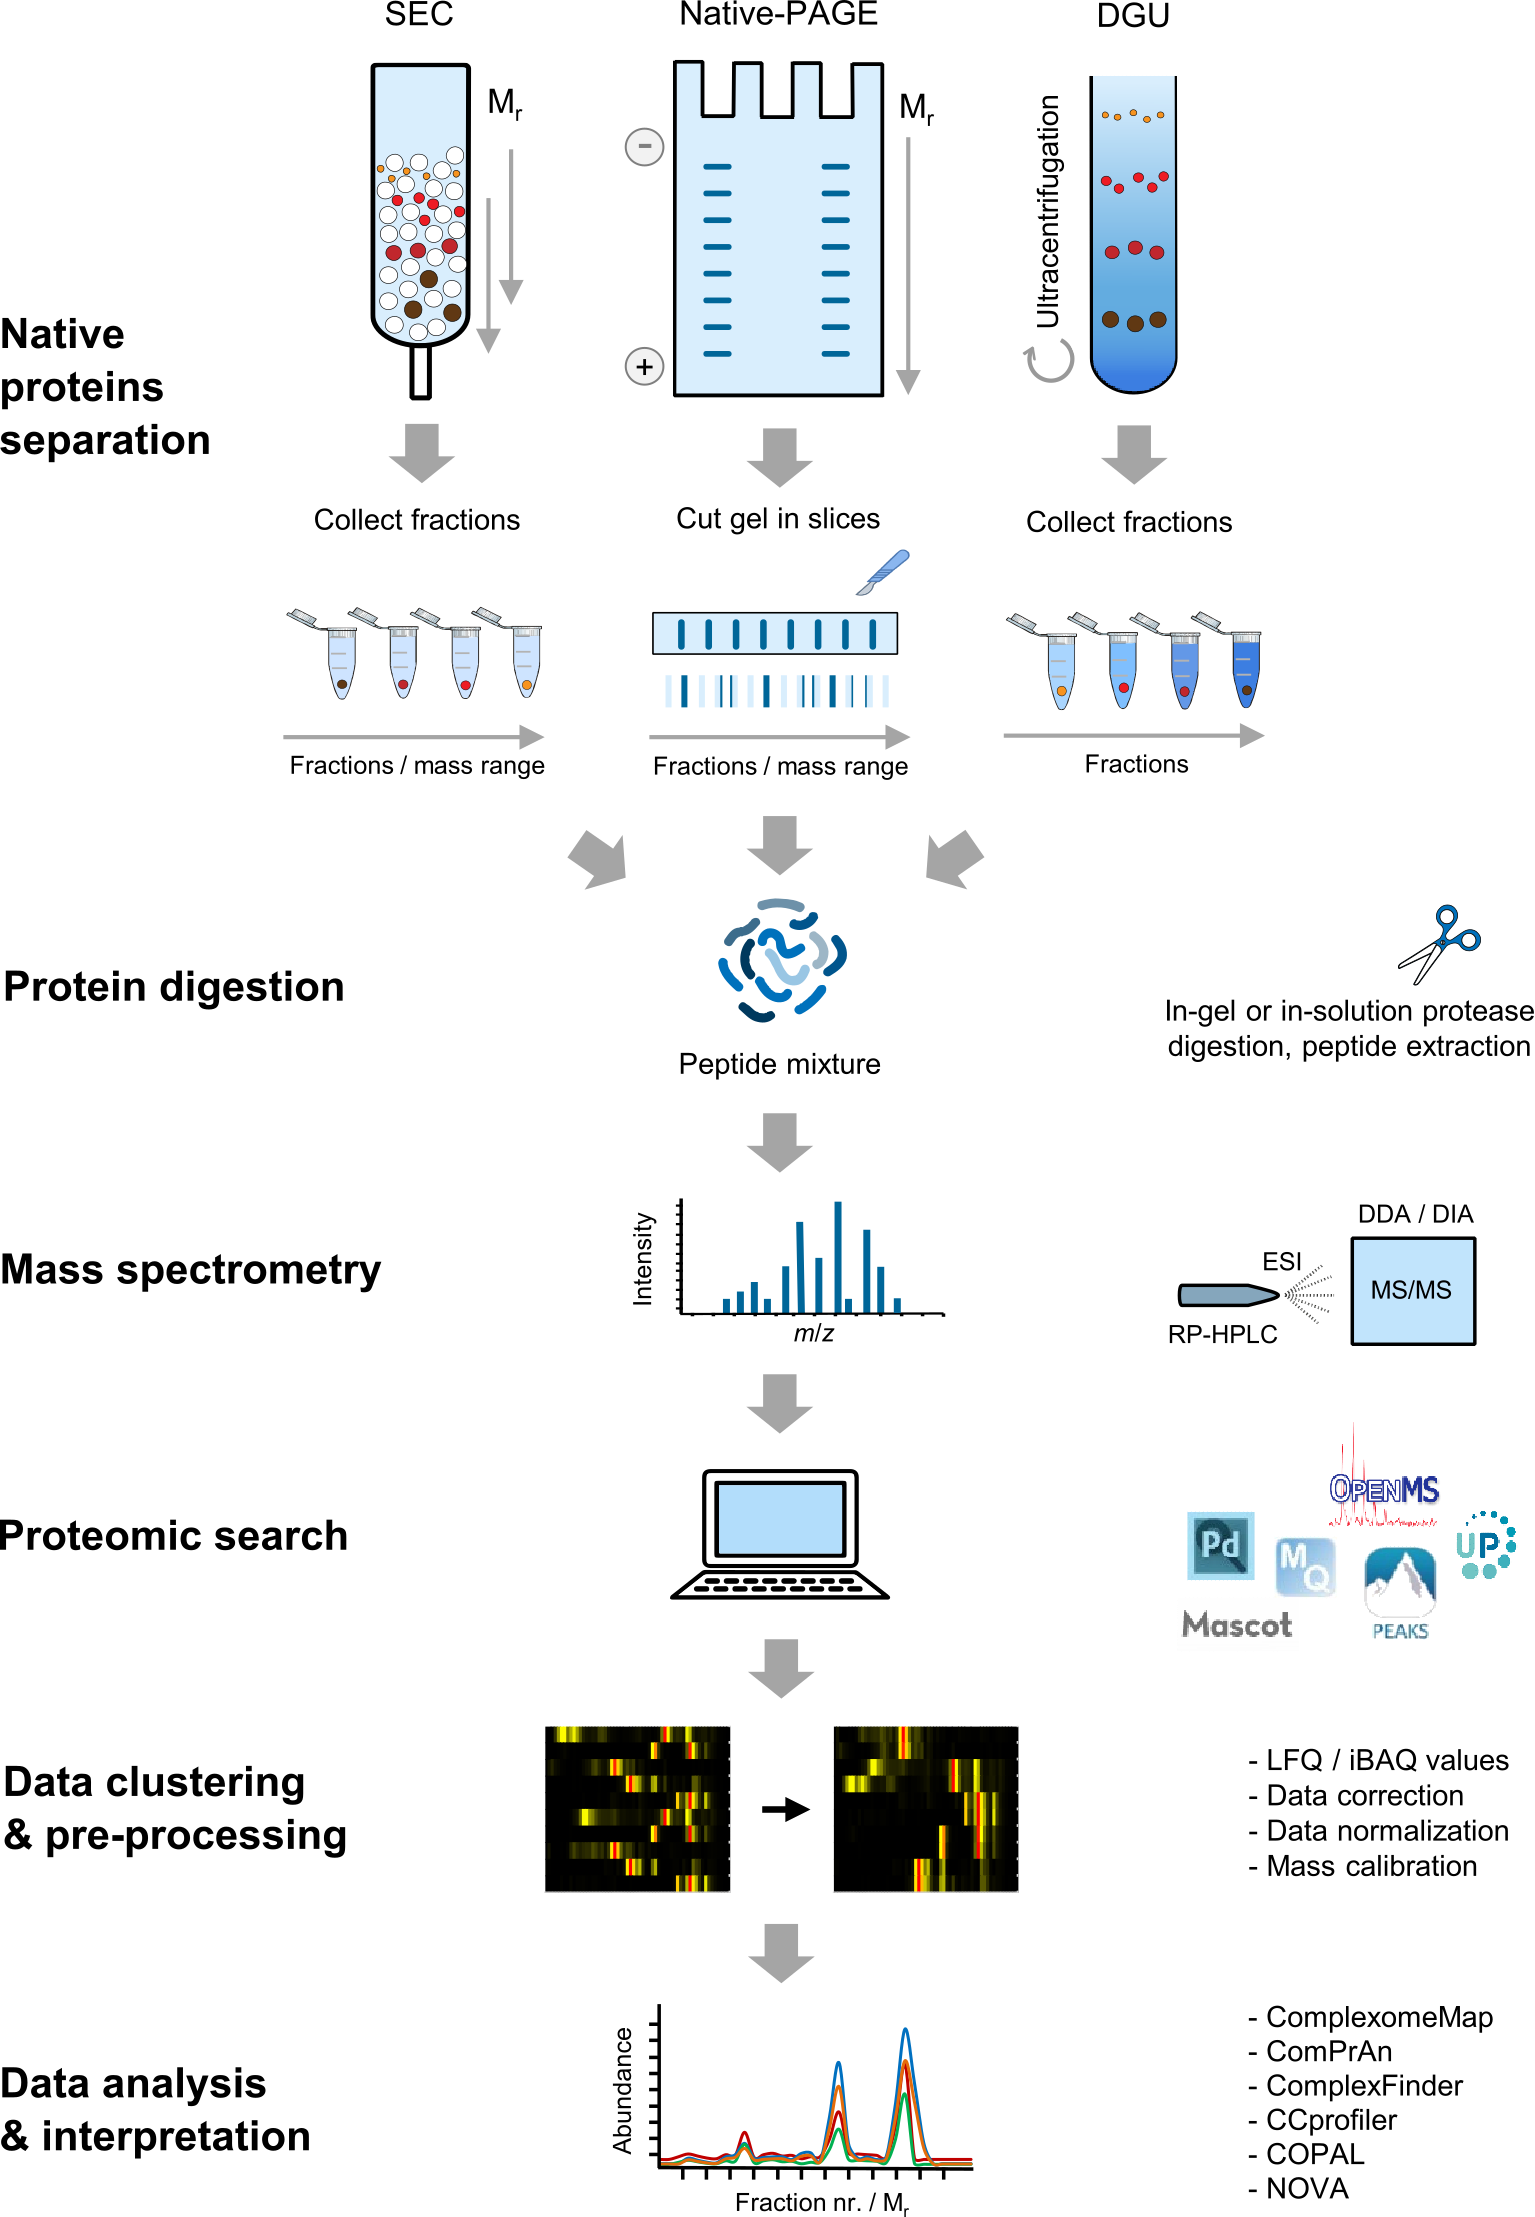
\includegraphics[width=0.9 \textwidth]{Chapter.1/Figures/Figure5.png}
    \caption{Figure Legend on next page}
    \label{fig:fig5}
\end{figure*}
\addtocounter{figure}{-1}
\begin{figure*}[ht!]
    \caption{\textbf{Overall workflow of complexome profiling (CP).} After collection, homogenization and fractionation of biological materials, proteins are separated by either native polyacrylamide gel electrophoresis (PAGE), size exclusion chromatography (SEC) or density gradient ultracentrifugation (DGU) for CP studies. The obtained protein-containing fractions are individually digested with specific proteases. Resultant peptides are extracted, cleaned and usually separated by reversed-phase high-performance liquid chromatography (RP-HPLC) followed by tandem mass spectrometry (MS/MS) analysis. MS data can be acquired in data-dependent or data-independent modes, DDA or DIA, respectively. Next, a proteomic search is performed to match obtained MS spectra against proteome databases using a variety of available software. Icons of the most popular tools used for CP studies are shown (see \textbf{\autoref{sec:CP_MS_intro}}). Protein abundance profiles are further obtained by plotting LFQ/iBAQ values against the number of fractions. The list of identified protein groups is computationally sorted based on similarities of the abundance patterns across fractions; e.g. hierarchical clustering. Prior to analysis, complexome data are pre-processed to account for protein loading/MS sensitivity differences. Data correction and normalization between samples are regularly applied. In SEC- and native-PAGE-based CP, a mass calibration can be implemented for a more meaningful biological dimension. Data can be analyzed by using available bioinformatic tools specifically created for CP (see \textbf{\autoref{ssec:CP_MS_ssec2}}). Some of these programs are shown in the figure. Figure adapted from \cite{Cabrera-Orefice_2022}.}
\end{figure*}
Proteins that are part of the same complex consistently cluster together since these show co-migration in the same fraction(s) and similar abundance profiles.
%
\subsection*{Different complexome profiling set-ups, one common goal}\label{ssec:CP_MS_ssec1}
As a ground-breaking “-omics” method, CP has been rapidly developing and spreading among the scientific community. It is thus not striking that in less than a decade, multiple strategies have complemented or even improved its scope. At the same time, several limitations of CP have been circumvented gradually by including novel MS-based strategies, specific adaptions in sample processing and new tools for data analysis. All variants of CP do share a common goal nonetheless: to unravel the composition of protein complexes, as well as their abundance, stabilities, apparent molecular masses and stoichiometries.\\
The most used CP workflow, currently referred to as “classic CP” \cite{Wittig_2021}, uses Blue Native-polyacrylamide gel electrophoresis (BN-PAGE) followed by MS identification. The main advantages of BN-PAGE are the relatively low amounts of biological material required and high-resolution separation of native proteins. BN-PAGE conditions keep proteins in similar native states to those occurring \emph{in vivo} \cite{Wittig_2006}. However, if the presence of Coomassie blue dye affects the stability of one or more protein complexes of interest, milder dye-free versions of native-PAGE can easily be used instead; e.g., high-resolution clear native-PAGE (hrCN-PAGE) \cite{Ladig_2011, Wittig_2007}. Native-PAGE is suitable for separation of proteins between $\sim$0.02-10 MDa. If the study requires interrogation of bigger protein complexes (>10 MDa), large pore BN-PAGE (LP-BN-PAGE) can be applied instead \cite{Heide_2012, Strecker_2010}.

After electrophoresis, entire gel strips are fixed and often cut into 32-70 slices followed by LC-MS/MS identification \cite{Giese_2021, Heide_2012, Senkler_2017, Vidoni_2017}. For CP analysis, slice numbers can be transformed into apparent molecular mass values by carrying out a calibration using standard proteins as exemplified in \cite{Heide_2012, Wittig_2010}. Molecular mass accuracy is optimized by using different sets of standard protein complexes, one for water-soluble proteins and the other for membrane proteins. On the whole, the more fractions collected the better resolution of the resultant profiles will be. In 2016, Müller and co-workers developed cryo-slicing Blue Native-Mass Spectrometry (csBN-MS), which helped increase the resolution, accuracy and quantification of the complexome profiles by slicing the BN-lanes in 230 pieces as well as optimizing MS analysis and protein identification \cite{Muller_2016}. The resolution of complexome profiles obtained from \(\leq\) 30 slices would not be suitable to unambiguously assign protein interactions.

Besides native-PAGE, size exclusion chromatography (SEC) and density gradient ultracentrifugation (DGU) have been implemented in different CP setups. Using SEC, native proteins are separated by filtration through a gel matrix (resin), which consists of spherical porous beads of different sizes depending on the desired range of molecular masses \cite{Burgess_2018}. Elution of heavier proteins is faster than the lighter ones by this method. Apparent molecular masses of eluted fractions can be determined with proper standard mixes; although the mass calibration is more accurate for globular proteins \cite{Hong_2012, Korepanova_2012}. SEC resins are suitable for separating proteins in a wide range of molecular masses; e.g. 1-700 kDa (SephadexTM, SuperdexTM); 5-5000 kDa (SuperoseTM) and 0.01-40 MDa (SepharoseTM). The number of fractions that can be collected after SEC is comparable to those aforementioned. For example, in the recently introduced SEC-SWATH-MS approach \cite{Heusel_2019}, 81 fractions were collected, subjected to MS identification and examined by complex-centric proteome analysis. This CP setup led to higher sensitivity and accuracy in protein quantification, less noise, and validation of protein interactions. SEC has been particularly useful in CP studies characterizing large protein complexes, such as nuclear components \cite{Connelly_2018}. However, key limitations of SEC-involving CP setups would be the larger amounts of biological material required, loss of protein interactions by dilution, formation of self-oligomers and inadequate identification of membrane and low abundant protein complexes \cite{Burgess_2018, Heusel_2019, Iacobucci_2021}.

On the other hand, DGU uses solutions of different densities made of glycerol, sucrose, cesium chloride, iodixanol or Ficoll\textsuperscript{®} through which protein complexes are separated based on their sedimentation rates, where heavier complexes sediment faster. DGU is an excellent technique for separating large protein complexes, ribosomes, membrane vesicles and subcellular organelles. DGU is also suitable to separate cleared cell lysates as well as immunoprecipitation (IP)-captured protein complexes \cite{Caudron-Herger_2019, Lee_2013}. After separation, most of resolved protein complexes remain in near-native states. In a recent study, a reliable DGU-based CP variant, referred to as quantitative density gradient analysis by mass spectrometry (qDGMS) has been developed to study the human mitoribosome \cite{Palenikova_2021a}. qDGMS combines stable isotope labeling by amino acids in cell culture (SILAC) and DGU followed by fractionation and LC-MS/MS analysis. SILAC is a MS-based technique that quantifies the differences in protein abundance/expression among biological samples \cite{Ong_2002}. In conventional SILAC, two different cell lines/strains are cultured using media supplemented with either “heavy” or “light” essential aminoacids that are labeled with non-radioactive isotopes (e.g., 13C, 2H, 18O, 15N) or unlabeled, respectively \cite{Geiger_2011}. The specific labeled aminoacids are hence incorporated into all cell proteins during cell growth. Proteins of cell lysates/fractions obtained from the two samples are mixed (1:1), digested and analyzed together by LC-MS/MS. The isotope-labeled peptides appear in MS spectra as pairs with identic chemical composition but different masses. Ratios of intensities for the many identified peptide pairs thus denote the respective changes in protein abundance between samples. Incorporation of SILAC not only in qDGMS but also in classic CP allows duplexing, MS time-saving and, most important, higher accuracy of quantification in proteomic analysis of two experimental conditions \cite{Palenikova_2021a, Palenikova_2021b}.

A major challenge of DGU relies on retrieving of fractions without manual disturbance of the resolved layers. To account for this issue, several strategies and devices have been developed, including commercially available automatic fractionators and freezing the gradient after centrifugation followed by cryo-slicing to fractionate samples consistently \cite{Yu_2016}. Location of resolved proteins by DGU is considerably more spread when compared to native-PAGE or SEC, which means that increasing the number of fractions does not necessarily lead to higher resolution. Furthermore, sedimentation rates do not only depend on molecular masses of protein particles but also on shape and densities from both the particles and fluid used for making the gradient \cite{Cole_2008}. For these reasons, co-migration of identified proteins by this CP setup does not immediately represent actual associations rather than merely similar sedimentation rates.
%
\subsection*{Complexome profiling data analysis and visualization} \label{ssec:CP_MS_ssec2}
Huge output files are obtained in CP studies after protein searches, which usually contain all data necessary for further analysis, including identified protein groups, unique peptides, sequence coverage, MS/MS counts, scores, LFQ/iBAQ values from each fraction, etc. The most common visualizations of a complexome profile are heatmaps accompanied by line charts plotting the LFQ/iBAQ values throughout the fractions. Complexome profiles of a short set of proteins can be manually generated and analyzed. Yet, the large volume of protein identifications in CP datasets makes full manual inspection impractical. In the last years, several tools have been specifically designed for automated processing and exploration of CP datasets.
ComplexomeMap has been developed as an online public platform for mining the mitochondrial complexome of plants \emph{Arabidopsis thaliana} and \emph{Viscum album} \cite{Senkler_2017}. NOVA is a user-friendly software to perform cluster analysis, mass calibration, normalization, visual inspection, links to protein databases and comparison of experimental conditions \cite{Giese_2015}. The software COPAL has proven helpful for analyzing multiple CP datasets, aligning experimental replicates and detecting significantly affected protein complexes \cite{Van_Strien_2019}. It also generates files that can be directly used for gene set enrichment analysis. ComPrAn, a Shiny R app, has been developed for analyzing qDGMS data; this tool enables analysis of peptide-level data, normalization, clustering, visualization options and a graphical user interface \cite{Palenikova_2021a}. In addition, ComPrAn is particularly useful to analyze proteomic data obtained from SILAC-treated samples. ComplexFinder, a Python-based software suit, has recently been released to analyze fractionation of native protein complexes, particularly from BN-PAGE- or SEC-based CP experiments \cite{Nolte_2021}. This tool allows machine learning-based prediction of potential protein-protein interactions (PPIs) and high flexibility in CP data analysis. ComplexFinder also provides improved peak-centric quantification and kinetic modelling, protein connectivity networks and compatibility with different quantification strategies. CCprofiler is a robust R package for analyzing co-fractionation MS datasets, which has been originally designed for SEC-SWATH-MS \cite{Heusel_2019}. CCprofiler and its web interface, SECexplorer, offer multiple functions, such as quality control and filtering for less erroneous assignment of protein interactors, usage of curated reference datasets, protein quantification, protein- and complex-centric data analysis and visualization.
Other software available for proteomic and interactome analysis can also be used for CP data processing. For instance, free tools such as Perseus \cite{Tyanova_2016b}, PrInCE \cite{Stacey_2017} and EPIC \cite{Hu_2019} may provide suitable options for visualization, protein quantification, statistical analysis, prediction of PPIs from co-fractionation data, obtention of supporting info from public repositories and/or cross-omics comparisons.
%
\subsection*{Complexome profiling as a tool to investigate mitochondrial protein complexes} \label{ssec:CP_MS_ssec3}
Complexome profiling as a tool to investigate mitochondrial protein complexes
Mitochondria are traditionally known as the eukaryotes` “powerhouses” since they contain all the enzymes required to generate ATP via the oxidative phosphorylation (OXPHOS) pathway. This process is catalyzed canonically by four respiratory chain complexes (I, II, III and IV) and a F1FO-ATP synthase (complex V). Complexes I, III and IV couple the energy released during electron transfer to oxygen to the generation of an electrochemical gradient of protons across the inner mitochondrial membrane (IMM). The proton gradient not only drives the synthesis of ATP, but also other processes such as metabolite transport, protein import, redox and Ca2+ homeostasis, fusion/fission, signaling and cell death. These organelles do also contain their own genome, also known as mitochondrial DNA (mtDNA), which encodes for a few but essential subunits of OXPHOS complexes. The roles of mitochondria are thus not limited to their energy duties. These organelles are multi-functional “hubs” critical to almost every cell process.
Despite of the great progress in molecular characterization and structure elucidation of numerous mitochondrial protein complexes, mostly OXPHOS- and mitoribosome-related proteins, a large number of mitochondrial PPIs remain elusive. In the last years, however, CP has proven valuable for identifying novel protein interactors, validating previous results and shedding light on intricate assembly pathways. In this section, we summarize these findings and describe how CP has boosted the analysis of protein complexes in the mitochondrial research field. Expectedly, most of these findings are again related to components or mediators of the assembly of OXPHOS complexes, energy metabolism-linked proteins and mitoribosomes.

The first groups that established CP have also been interested in the many features of OXPHOS and in particular of complex I (CI). CI is the largest redox enzyme of the mitochondrial respiratory chain constituted by $\sim$45 subunits depending on the species. CI generates proton-motive force driven by the transfer of electrons from NADH to ubiquinone \cite{Hirst_2013}. Although the redox features and composition of mitochondrial CI in several species were already known by the start of the 2010s, major queries on this enzyme had yet unresolved: its entire 3D structure, its energy-conversion mechanism and how it assembles. To help tackle the last one, the formal introduction of CP by Heide and co-workers was useful to identify TMEM126B interacting with the known CI assembly factors NDUFAF1, ECSIT and ACAD9 \cite{Heide_2012}. \emph{TMEM126B} knockdown in 143B osteosarcoma cells led to $\sim$95 \% specific decrease in CI-containing supercomplexes, i.e. supramolecular associations of complexes I, III and IV. These results thus proposed TMEM126B as a CI assembly factor. In an earlier report using HEK293 cells, Wessels and co-workers identified with a similar approach two other assembly factors of CI: C6ORF66 and C3ORF60 \cite{Wessels_2009}, currently known as NDUFAF4 and NDUFAF3, respectively. In this study, mitochondrial proteins were separated by BN-PAGE followed by LC-MS/MS identification, but comparison of migration patterns was limited to the use of PCP.

A few years later, a dynamic CP strategy was successfully implemented to describe the step-by-step integration of the subunits, assembly factors and the different assembly intermediates of human CI \cite{Guerrero-Castillo_2017a}. The authors used CP data from time-based mitochondrial translation recovery to describe a number of assembly intermediates of CI accumulating at various timepoints after removal of chloramphenicol, a reversible inhibitor of mitoribosomes \cite{Ugalde_2004}. These data corroborated the long time proposed modular assembly pathway of CI, which basically involves the coordinated formation and pre-assembly of its functional modules, N, Q, PP and PD, before forming the entire enzyme. This study also provided insight into the specific involvement of earlier reported assembly factors and novel interactors. Complex IV (CIV) assembly-related chaperone COA1 and TMEM186 were clearly found associated with membrane arm intermediates that also interact with TMEM126B, NDUFAF1 and ECSIT. At present, all these proteins have been recognized as true components of the so-called mitochondrial CI assembly (MCIA) complex \cite{Formosa_2020}. ATP5SL clustered with FOXRED1, another CI assembly factor. However, ATP5SL disruption did not lead to CI deficiency \cite{Andrews_2013} and its involvement in the assembly pathway is thereby unclear. Complex V assembly-involved protein TMEM70 was also identified in assembly intermediates of CI. To further explore the putative role of TMEM70 on CI assembly, Sánchez-Caballero and co-workers performed a study including proximity-dependent biotin identification (BioID), co-evolution analyses and CP \cite{Sanchez-Caballero_2020}. In this study, TMEM70 was found in close contact with subunits of complexes I and V, as well as the small mitoribosome subunit. The absence of TMEM70 resulted in slight depletion of fully assembled CI and accumulation of assembly intermediates of the distal part of the membrane arm of CI, whereas mature complex V (CV) content was $\sim$70 \% lower than in the control cell line. These authors showed TMEM70 as a non-essential assembly factor of complexes I and V, and proposed a possible role in tethering mitoribosomes to the IMM during translation.
Apart from studies in human cells, CP has also been used to study the role of several accessory subunits of CI in different models. For example, Kmita and co-workers analyzed the assembly of CI in a deletion strain of the yeast \emph{Yarrowia lipolytica} lacking the Zn2+-containing subunit NUMM/NDUFS6 \cite{Kmita_2015}. Absence of this subunit did not prevent formation of the entire CI, since a lower enzyme content and higher fraction of peripheral arm subcomplexes were observed. Unexpectedly, the almost fully assembled CI contained the assembly factor N7BML/NDUFAF2 bound instead of accessory subunit N7BM/NDUFAF12. Moreover, Angerer et al. implemented CP in a study on the mitochondrial acyl carrier proteins (ACPM) 1 and 2, which are accessory subunits of CI and contain LYR motifs \cite{Angerer_2014}. Although ACPM1/2 are predominantly associated to CI, ACPM1 was also found as a free protein in the matrix and forming a complex with LYRM4(ISD11)/NFS1 involved in iron-sulfur cluster biosynthesis. Furthermore, two different groups in parallel unveiled the existence of two isoforms of the peripheral arm subunit NDUFV3 of CI in mammals \cite{Bridges_2017, Guerrero-Castillo_2017b}. An extra exon present in gene \emph{NDUFV3} can be alternative spliced, hence generating short and long isoforms of $\sim$10 and $\sim$50 kDa, respectively. CP helped find a different expression of these isoforms in different tissues of bovine, mouse and rat as well as in cultured human cells. The canonical short isoform was predominantly identified in heart and skeletal muscle, whereas the large isoform was the foremost isoform in liver, brain and lung tissues. Both NDUFV3 isoforms can also be expressed at the same time and correctly assembled onto CI in some tissues; yet, one isoform predominated in each case.

Other OXPHOS complexes and their chaperones have also been explored by CP. Singhal et al. identified the product of ORF \emph{YDR381C-A} as an assembly factor of yeast complexes III and IV \cite{Singhal_2017}. This protein was renamed as cytochrome \emph{c} oxidase interacting protein 1 (Coi1), which occurs only in fungi. Deletion of Coi1 resulted in severe alteration of mitochondrial function, diminished amounts of CIV-associated heme, defective assembly of complexes III, IV and their supercomplexes, as well as accumulation of assembly intermediates. Vidoni and co-workers reported that the short isoform of myofibrillogenesis regulator 1 (MR-1S) associates with chaperones PET100 and PET117 to mediate human CIV assembly \cite{Vidoni_2017}. Authors implemented not only CP to study assembly intermediates accumulated in control and \emph{MT-CO3} mutant cybrids, but also SILAC and quantitative MS.\\
CP has been helpful to better understand the formation of supercomplexes or respirasomes. The specific factors for mediating this process remain unclear. COX7A2L, also known as SCAFI, has been shown critical for the association of complexes III and IV \cite{Perez-Perez_2016}. Its putative involvement in larger respirasome formation has also been reported \cite{Lapuente-Brun_2013}. To better understand the role of SCAFI, Férnandez-Vizarra et al. explored the mitochondrial complexome of a SCAFI knockout human cell line by SILAC-based CP \cite{Fernández-Vizarra_2021}. Absence of SCAFI resulted in marked loss of supercomplex III2-IV, whereas CI-containing respirasomes were not affected. In contrast, authors showed that $\sim$70 \% of respirasomes contained COX7A2 in either human cell line analyzed. This discrepancy has apparently been related to a tissue-specific expression of the two isoforms \cite{Lapuente-Brun_2013}. On the other hand, Protasoni and co-workers demonstrated that absence of a fully assembled complex III (CIII) in a MT-CYB-deficient human cell line stalled CI biogenesis by preventing the integration of its N-module \cite{Protasoni_2020}. Although substantial accumulation of partially assembled Q/P intermediate was observed by SILAC-based CP, a slight fraction of CI could still be detected. Reasonably, respirasome assembly was totally lost in the mutant. Besides, assembly of CIV was affected since several COX subunits were found associated with CIII sub-assemblies; hence interfering their correct assembly. It has thus been proposed that human complexes I, III and IV assemble in a cooperative fashion, where CIII seems to be central.

Mitochondria are characterized by a highly folded IMM. These folds, called cristae, have emerged as dynamic compartments whose shape and dimensions influence structure and functioning of the OXPHOS system \cite{Cogliati_2016}. A key player in shaping cristae appears to be the MICOS complex, which also interacts with the sorting and assembly machinery (SAM) complex from the outer mitochondrial membrane (OMM) \cite{Huynen_2016}. Interaction of these two complexes constitutes the mitochondrial intermembrane space bridging (MIB) complex \cite{Ott_2015}. Since its relatively recent discovery \cite{Harner_2011}, much of what we know about the MICOS complex has been derived from CP-based studies. For instance, Weber and co-workers identified apolipoprotein O (APOO/MIC26) and apolipoprotein O-like protein (APOOL/MIC27) as potential components of the human MIB complex \cite{Weber_2013}. Huynen and co-workers described the composition and apparent masses of the fully assembled MIB complex (2.2-2.8 MDa) and other putative assembly intermediates, e.g. the free MICOS complex ($\sim$700 kDa) \cite{Huynen_2016}. Anand et al. identified MIC13 (QIL1) as a novel MICOS complex subunit \cite{Anand_2016}. Deletion of MIC13 resulted in a smaller albeit still assembled MICOS complex while having no effect on integrity of OXPHOS complexes. They also demonstrated a disruptive effect of MIC13 deletion on cristae morphology accompanied by reduced respiratory capacity. The same group used a similar approach to characterize MIC26 and MIC27 \cite{Anand_2020}. They showed negative effects on CV stability as well as cristae morphology defects both of which were much more pronounced in the double knockout than either single knockout, suggesting overlapping roles. Assembly of other MICOS components was however unimpeded by MIC26/27 knockouts, proposing these proteins are not essential for its assembly or stability. The link of MICOS components to CV was further explored by Eydt and co-workers \cite{Eydt_2017}, showing that MIC10 comigrates with CV dimers. Additionally, they presented evidence that MIC10 acts antagonistically to MIC27 in negatively controlling CV oligomerization, while MIC27 appears to be a positive regulator. A recent paper by Bock and co-workers reported the interaction of  PGC-1- and ERR-induced regulator in muscle 1 (PERM1) with multiple components of the MICOS/MIB complex as well as vimentin and ankyrin B in skeletal muscle from mouse \cite{Bock_2021}. These findings suggested a novel mechanism to help understand not only the interconnection of mitochondria and sarcolemma but also mitochondria-cytoskeleton associations as well as the organization of a functional mitochondrial network in this tissue. Taken together CP has greatly aided our understanding of MICOS/MIB complex composition, the role of individual subunits and its interaction with OXPHOS complexes.

The IMM contains other key protein complexes involved in proteolytic events, fusion/fission of mitochondrial membranes, regulation of cristae morphology and cell signaling. Some of these proteins belong to the SPFH (stomatin, prohibitin, flotillin and HflC/K) family and usually arrange as large scaffolds. To have a clearer picture, Wai and co-workers implemented CP to unveil the interaction partners of stomatin-like protein 2 (SLP2) and at least two proteases, PARL and YME1L, in immortalized embryonic fibroblasts mitochondria \cite{Wai_2016}. SLP2 works as a regulator of PARL, which also modulates other proteins such as PGAM5, PINK1 and OMA1. These interactions were suggested to occur in defined sites of the IMM and related to mitochondrial proteostasis, dynamics and cell survival. Similarly, Konig and co-workers identified MAIP1 (C2Orf47) as a novel \emph{m}-AAA protease-binding protein in complexome profiles \cite{Konig_2016}. MAIP1 was shown essential for regulating the assembly of subunit EMRE into mitochondrial Ca2+ uniporter (MCU) complexes.

CP has also played an important role in the field of plant and parasite mitochondrial biology. Using CP, Senkler and co-workers performed a systematic characterization of mitochondrial complexes in the plant \emph{Arabidopsis thaliana} \cite{Senkler_2017}. CP data were also useful to update the subunit composition of OXPHOS complexes and identifying respective assembly intermediates. This group then used the same approach on mitochondria from the mistletoe \emph{Viscum album}, revealing a highly unusual OXPHOS system \cite{Senkler_2018}. This species completely lacks CI, the only multicellular eukaryote to date with this distinction; instead, \emph{Viscum album} contains alternative NAD(P)H oxidoreductases. This species also expresses an alternative oxidase and its complexes III and IV are firmly associated as supercomplexes. In comparison to \emph{Arabidopsis thaliana}, the abundance of complexes II and V was particularly low, suggesting a shift in stoichiometry of the OXPHOS complexes in the IMM of this plant. Rugen and co-workers took a more focused CP strategy to investigate the composition of the mitoribosome in \emph{Arabidopsis thaliana} \cite{Rugen_2019}. Utilizing LP-BN-PAGE- and DGU-based CP setups, several non-conventional proteins were found attached to the mitoribosome, mostly from the class of pentatricopeptide repeat proteins that seem to be involved in RNA processing and protein maturation. Presence of these additional interactors results in a larger mitoribosome with unusual large and small subunits of $\sim$3 and $\sim$5.7 MDa, respectively. Additional functions are thus likely incorporated into the plant mitoribosome.

Due to their extreme divergence, apicomplexan parasites of the genera \emph{Plasmodium} and \emph{Toxoplasma} that cause the infectious diseases malaria and toxoplasmosis, respectively, remain poorly understood. In fact, more than one-third of their genes still lack any functional annotation \cite{Aurrecoechea_2009, Harb_2020}. To help narrow this gap, Evers et al. and Maclean et al. obtained evidence for highly divergent composition of the mitochondrial OXPHOS complexes in \emph{Plasmodium falciparum} and \emph{Toxoplasma gondii}, respectively \cite{Evers_2021, Maclean_2021}. More than 30 novel subunits across complexes II, III, IV and V with no recognizable orthologs outside of the myzozoan phylum could be identified by CP. These novel subunits did not only replace subunits typically observed in standard models, but also increased the size of \emph{Plasmodium falciparum} OXPHOS complexes by around 50 \%, 50 \%, 130 \% and 70 \% as compared to complexes II, III, IV and V from mammalian mitochondria, respectively. This was consistent with the observations in \emph{Toxoplasma gondii}, thus making apicomplexan OXPHOS complexes the largest described to date. Furthermore, abundance of OXPHOS complexes was $\sim$32 fold increased in the transmissible gametocyte stages compared to the pathogenic asexual stages of \emph{Plasmodium falciparum} \cite{Evers_2021}. This finding offered protein-level support for the long-standing hypothesis that malaria parasites undergo a metabolic switch towards mitochondrial catabolism to facilitate their transmission back to the insect vector \cite{MacRae_2013}. Despite its relatively recent introduction to the field of parasite research, CP has already provided valuable data for mapping a number of previously unknown interactors to protein complexes and biological processes. As these novel additions are unlike what is known from standard models, it opens the door for new discoveries, even in pathways as fundamental as respiration.
%
\section{Combining XL-MS and CP-MS for the structural analysis of protein complexes in mitochondria}
Over the last decade, through advances in mass spectrometry, chemical cross-linkers and data base search strategies cross-linking mass spectrometry (XL-MS) has emerged as a powerful technology for interactome and structural biology studies in mitochondria \cite{Hevler_2021b, Liu_2018, Ryl_2020, Schweppe_2017}. Notwithstanding, the diverse protein complex landscape within mitochondria, where some proteins are found across several co-occurring complexes (e.g. respiratory super-complexes) \cite{Letts_2016, Rugolo_2021, Schägger_2000, Wu_2016}, substantially complicates the structural analysis. While XL-MS provides information about physical interactions within a complex, its exact stoichiometry cannot be confidently assigned. Knowing the exact stoichiometry of a complex is essential to guarantee accurate cross-linking guided structural modeling of protein complexes. For this reason, CP and XL-MS are highly complementary and could provide valuable insights into the macromolecular organization of the mitochondrial complexome. As shown in chapter 2 of this thesis, combining CP and XL-MS data enabled detailed atomic modeling of monomeric complex IV (COX) associated with dimeric apoptosis-inducing factor 1 (AIFM1) \cite{Hevler_2021b}. CP analysis was indeed helpful to determine the stoichiometry of this complex and validating the interaction. Combination of both approaches offers the possibility to cross-validate PPIs and to identify protein complexes that could be overlooked otherwise. Although actual scalability and throughput have not yet been addressed, combination of CP and XL-MS holds a great potential not only to better define the composition and states of protein complexes but also to help stabilize transient PPIs.

Besides knowing the exact complex stoichiometry, determination of the optimal concentrations of cross-link reagent and protein is strictly required to abate artifacts. To help circumvent this, in chapter 3 we describe a hybrid workflow termed in-gel cross-linking (IGX-MS) \cite{Hevler_2021a}. In this method, proteins are separated by BN-PAGE and the gel spots of interest are cut and incubated with a cross-linker, digested and further analyzed by LC-MS/MS. IGX-MS not only makes time-consuming experimental optimization steps (e.g. determining concentration of cross-linkers, optimal buffer system, etc.) nearly obsolete but also decreases the required protein amounts as well as undesired over-length cross-links. In contrast to classical in-solution XL-MS workflows, IGX-MS allows the differentiation of conformation- and interaction-specific distance restraints as it has been shown for various mitochondrial complexes but also for plasma protein complexes, the mitotic checkpoint complex (MCC) as well as for different assemblies of the archaeal ammonia monooxygenase \cite{Fischer_2022, Hevler_2021a, Hodgskiss_2022, Lukassen_2021}. IGX-MS seems specially promising for future modeling studies that aim at characterizing co-occurring protein complexes with different stoichiometries or assembly states.
XL-MS has also been used to validate another CP-like setup that includes protein separation by SEC, quantitative MS analysis, cryo-electron microscopy (EM) and computational modeling. This structural proteomics approach allowed simultaneous description of the abundance, PPIs and structure profiling of 1/3 of the proteome of \emph{Chaetomium thermophilum} \cite{Kastritis_2017}. These results were integrated in a network map comprising 48 protein complexes and communities. This approach was also suitable to resolve the structure of the fatty acid synthase complex and its arrangements. Recent inclusion of image-processing workflows based on machine-learning methods opens the door to a much more robust data analysis, improved identification of PPIs, higher resolution in structure models and multi-scale molecular description of protein communities in situ \cite{Kyrilis_2021a}.
\newpage
\section*{References}
\bibliographystyle{Style_settings/bibstyle_pnas}
\bibliography{Chapter.1/chapter1_bib_form}

